\documentclass[../../main.tex]{subfiles}
\begin{document}
\chapter{Conclusion}
\label{ch:conclusion}

In this chapter, we present a summary and overview of the contributions made in this thesis on \textit{\gls{sl} Synthesis by a Decreasing Granularity System from AZee}. In Section~\ref{ch:conclusion:summary}, we summarize the main findings and insights from the research. In Section~\ref{ch:conclusion:contributions}, we highlight the publications and open-source implementations that have resulted from this work. In Section~\ref{ch:conclusion:key_insights}, we present key insights that have emerged from the research, including the importance of granularity in \gls{sl} synthesis and the relationship between language and motion. Finally, in Section~\ref{ch:conclusion:future}, we outline potential future directions for research in \gls{sl} synthesis, including enhancing the decreasing granularity model, expanding the capabilities of the AZee framework, and exploring real-time synthesis applications.

\section{Summary}
\label{ch:conclusion:summary}

This thesis explores innovative approaches to synthesizing \gls{sl} using a decreasing granularity system based on the AZee framework. The primary objective was to develop a system that could generate \gls{sl} sequences that are linguistically accurate and easier to reproduce, addressing a crucial need of empowering \gls{sl} communication technologies for the Deaf and Hard of Hearing communities.

In Chapter~\ref{ch:background_work}, we reviewed the foundational work in describing \gls{sl}s, and synthesis techniques, particularly focusing on synthesis from AZee. AZee provides a structured way to describe \gls{sl} at varying levels of granularity. However, existing methods often struggle to balance linguistic accuracy with ease of synthesis. 

Chapter~\ref{ch:avatar_creation_pose_synthesis} introduced our methodology to create a signing avatar, emphasizing the importance of rigging in realistic character animation. It presented a procedural rigging system tailored for AZee inside blender. The chapter discussed automating site generation and improving the rigging process with deformation, inverse kinematics (IK), and forward kinematics (FK) layers. It also introduced our algorithm for constraint-based posture optimization. Finally, the chapter evaluated the system’s animation quality and performance, highlighting the potential for future enhancements in \gls{sl} avatar animation. 

In Chapter~\ref{ch:multi_track}, the concept of multi-track and non-linear synthesis is introduced to improve \gls{sl} avatar animation. The chapter explores how multi-track control mimics natural human motion by preserving the dynamics of simultaneous gestures, facial expressions, and body movements. Non-linear synthesis ensures correct animation sequences and resolves conflicts between overlapping blocks. It discusses converting AZee Synced Scores into multi-track timelines and then solving for the posture using constraint-based  optimization. The chapter also highlights the integration of pre-animated blocks and evaluates the improvements in animation quality and flexibility using Blender's \gls{nle}.

In Chapter~\ref{ch:intermediate_blocks_pose_correction}, we discuss how synthesis can be improved using real world captured data. The generation of intermediate blocks in \gls{sl} synthesis is explored to improve the natural flow between signs. By leveraging motion curves and AZee templates, the chapter discusses how transitions can be enhanced in a multi-track representation. It introduces reusable motion templates to create smooth, realistic animations for some common AZee rules. The chapter also explores use of pose correction for \gls{sl} synthesis, focusing on improving naturalness and accuracy in \gls{sl} avatars. For this, we integrate a pose prior model, trained on a \gls{lsf} motion capture dataset, to guide the correction process using \gls{vae}. The chapter evaluates the results of both template-based interpolation and pose correction compared to previous methods, highlighting improvements in naturalness and coherence. It concludes with insights on limitations and potential future improvements in finger articulation and generalization of templates. 

Chapter~\ref{ch:facial_expressions} a method for synthesizing facial expressions using the AZee framework, focusing on action units from the \gls{facs} system to create blendshapes for animating signing avatars. It explores blendshape modeling, use of blendshapes with AZee, and templating facial expressions using motion curves to create dynamic and realistic facial expressions. The chapter evaluates the accuracy of synthesized expressions through subjective measures, demonstrating the potential of this approach for improving the realism of signing avatars.

\section{Contributions}
\label{ch:conclusion:contributions}

Work presented in this thesis has been the subject of the following publications:

\begin{enumerate}
    \item Paritosh Sharma, Michael Filhol. "Sign Language Synthesis using Pose Priors." In \textit{Proceedings of the 9th International Conference on Movement and Computing (MOCO '24)}, ACM, 2024, Utrecht, Netherlands.
    
    \item Paritosh Sharma, Camille Challant, Michael Filhol. "Facial Expressions for Sign Language Synthesis using FACSHuman and AZee." In \textit{SIGNLANG}, 2024.
    
    \item Paritosh Sharma, Michael Filhol. "Extending Morphs in AZee Using Pose Space Deformations." In \textit{2023 IEEE International Conference on Acoustics, Speech, and Signal Processing Workshops (ICASSPW)}, IEEE, 2023, pp. 1-5.
    
    \item Paritosh Sharma, Michael Filhol. "Intermediate Block Generation for Multi-Track Sign Language Synthesis." In \textit{Proceedings of the ACM SIGGRAPH/Eurographics Symposium on Computer Animation (SCA '23)}, ACM, 2023, Los Angeles, CA, USA.
    
    \item Paritosh Sharma. "A Layered Approach to Constrain Signing Avatars." In \textit{VISIGRAPP\_DC 2023}, Scitevents, Feb 2023, Lisbon, Portugal.
    
    \item Paritosh Sharma, Michael Filhol. "Multi-Track Bottom-Up Synthesis from Non-Flattened AZee Scores." In \textit{7th Workshop on Sign Language Translation and Avatar Technology (SLTAT 7)}, Jun 2022, Marseille, France.
\end{enumerate}

Apart from the above publications, one of the key contributions of this thesis is the open-source implementation of the synthesizer for AZee. The system extends the original AZee language model and integrates it with a decreasing granularity framework to synthesize signs directly in blender~\ref{fig:conclusion:azee_animator_interface}.

\begin{figure}[ht]
    \centering
    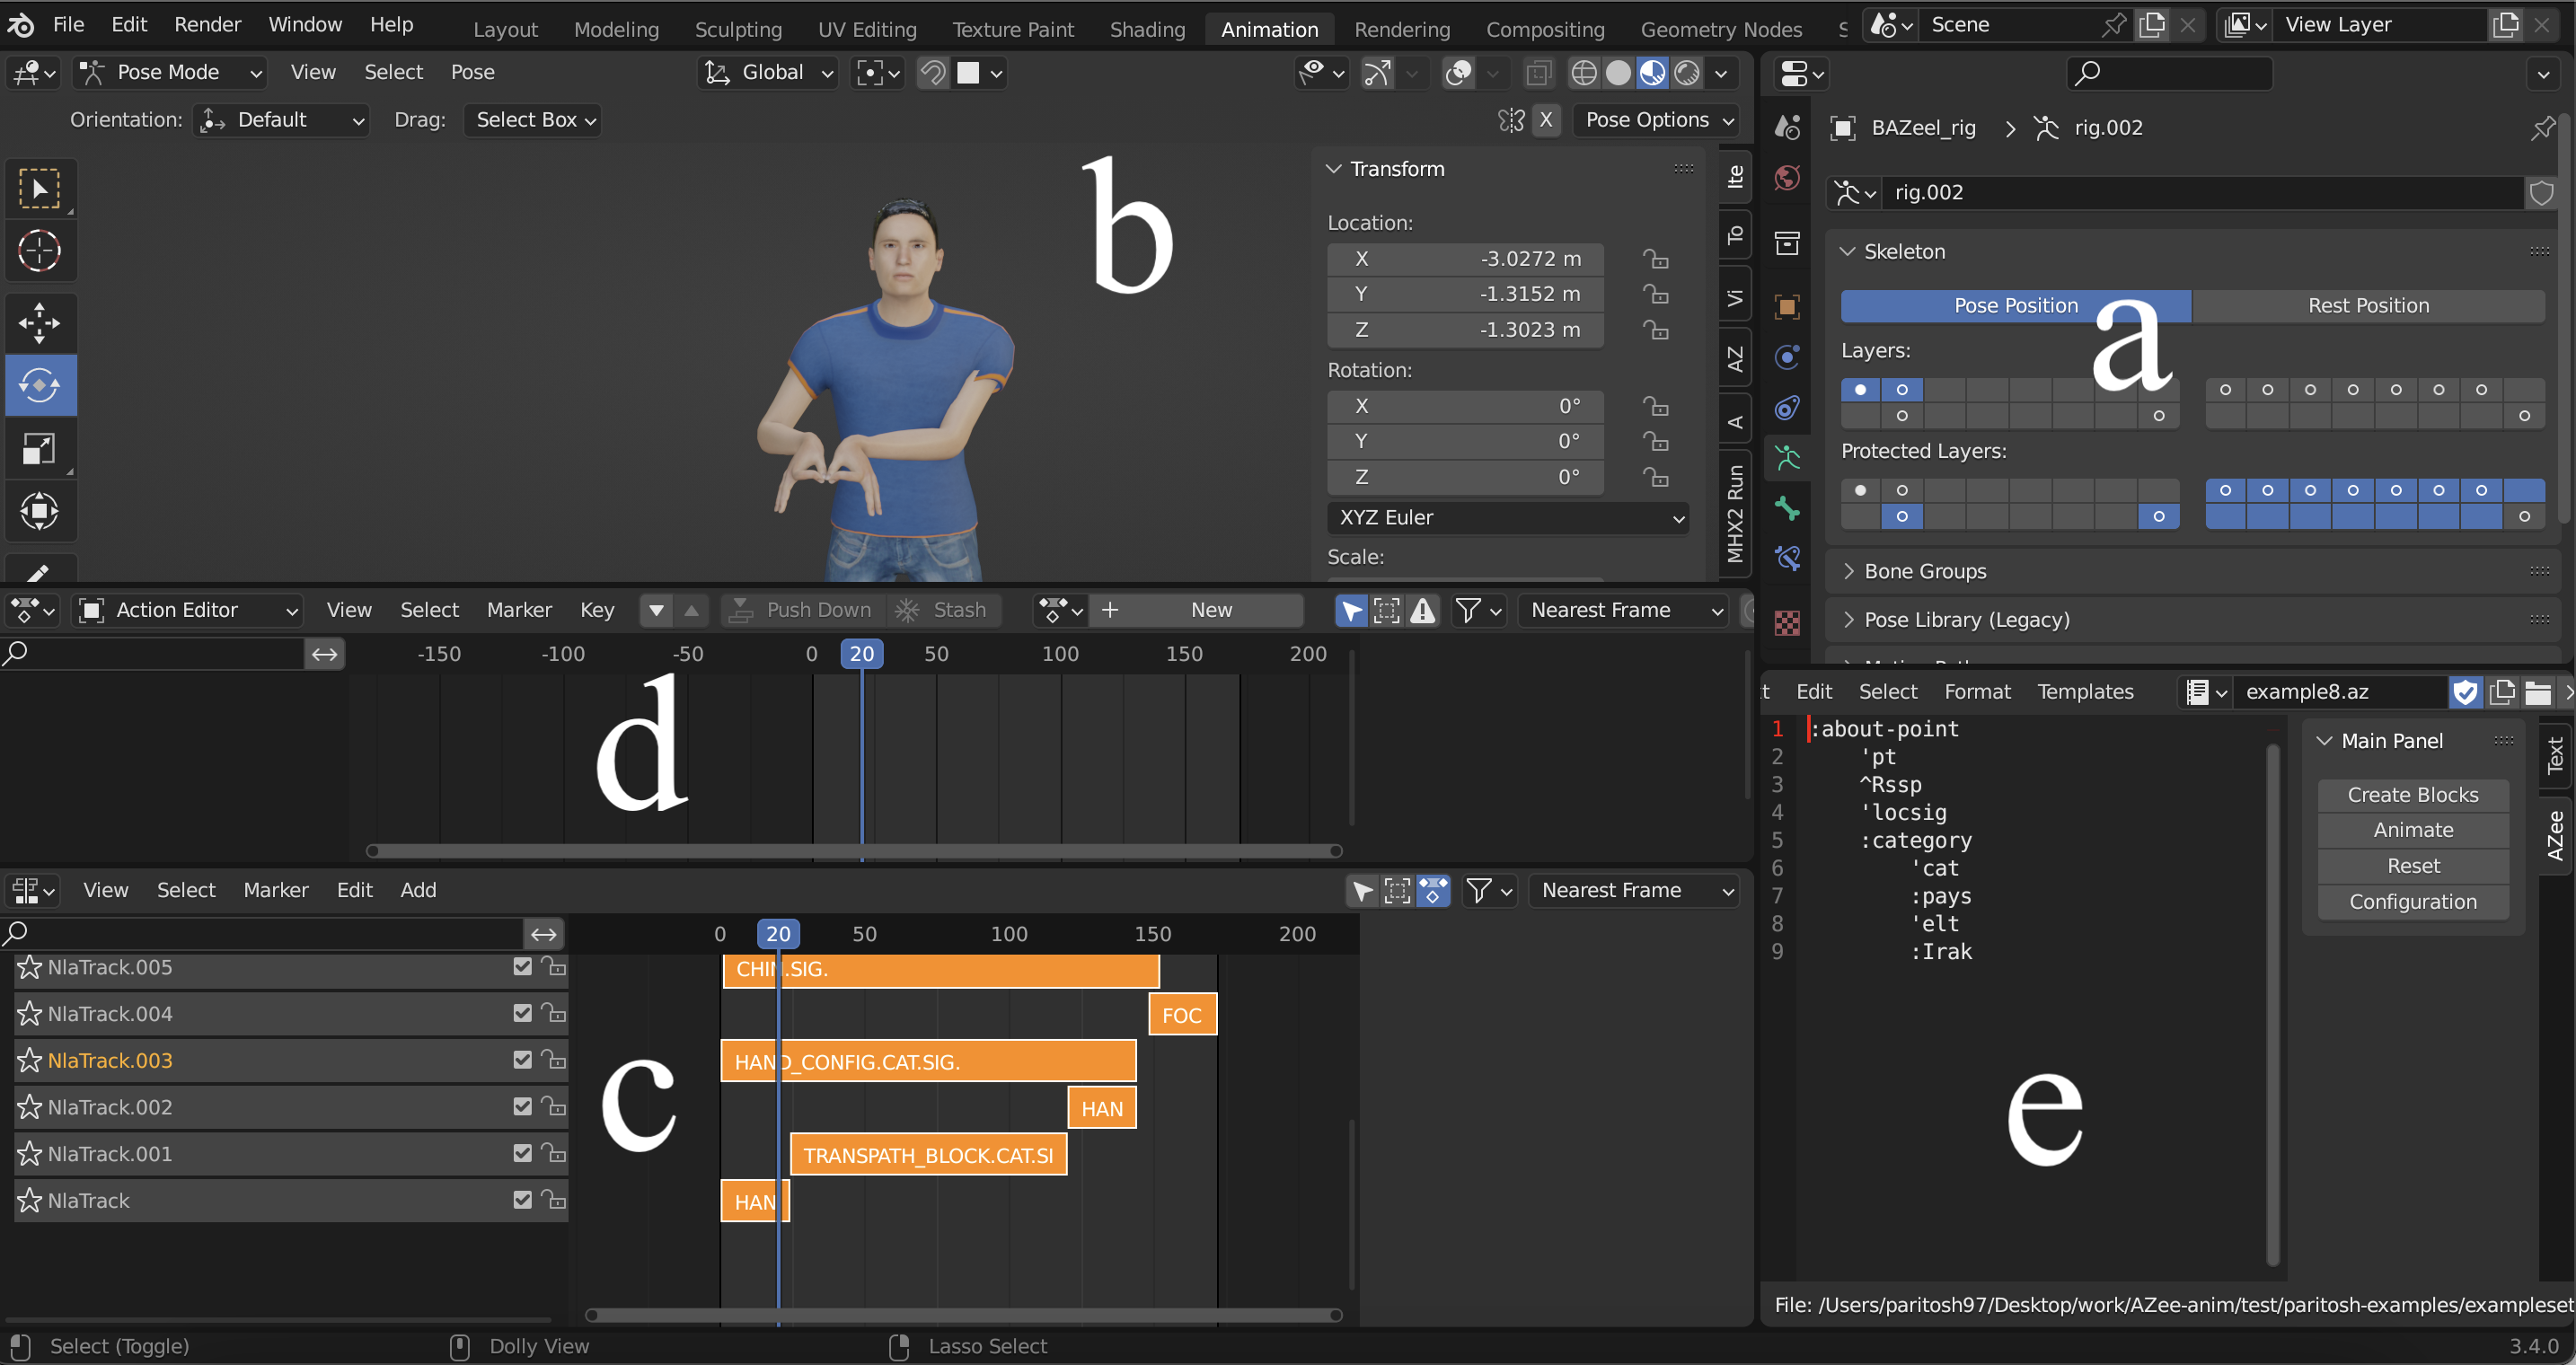
\includegraphics[width=0.8\textwidth]{chapters/conclusion/images/blender-interface.png}
    \caption{AZee animator interface}
    \label{fig:conclusion:azee_animator_interface}
\end{figure}

The animator interface allows users to write AZee code in a text editor and visualize the corresponding \gls{sl} animations in real-time. For this, the animator loads the AZee compiler as a python module and uses evaluates the generated AZee Scores directly on the avatar. The add-on uses blender's \gls{nle} to manage the animation blocks and transitions of the multi-track system. The system also supports facial expressions, intermediate blocks and pose correction.

\section{Key Insights}
\label{ch:conclusion:key_insights}

The research conducted in this thesis has yielded several key insights that can inform future work in \gls{sl} synthesis and related fields. These insights are summarized below:

\subsection{Granularity}
\label{ch:conclusion:key_insights:granularity}

This thesis highlights the concept of granularity in both \gls{sl} representation and synthesis. The term \emph{shortcut} refers to animating linguistic constructs at a higher level of granularity, enabling more natural synthesis while preserving linguistic accuracy, though this comes at the cost of finer control over the animation. Traditional research has typically mapped granularity directly to animations. In contrast, this thesis examines granularity at the posture level, offering a new perspective on \gls{sl} synthesis.

Much like how an artist rigs a character with various control points to manage movement, an AZee linguist employs a similar approach to structure \gls{sl} discourse. Each control point—whether an \gls{ik} placement, blendshape, pre-trained pose corrector, or FK rotation—can be seen as a linguistic construct with a certain granularity. This approach allows for the creation of expressive, linguistically accurate animations, offering a more detailed and flexible way to synthesize \gls{sl}.

\subsection{Language and Motion}
\label{ch:conclusion:key_insights:language_motion}

The AZee model offers a structured approach to describe \gls{sl}, which is crucial because it differs from simply translating \gls{sl} to or from a spoken or written language. While an AZee discourse has a one-to-one relationship with its corresponding \gls{sl} utterance, the utterance itself can have multiple equivalent translations. Both motion and language are temporal and exist in high-dimensional spaces, but the type of information they carry is different. Body motion operates in a visual space influenced by identity, surroundings, and physical laws, whereas spoken or written language is a human construct, independent of such factors. This distinction doesn't apply to \gls{sl}s, as their motion space is tied to their linguistic structure. Thus, while a common \emph{space} between an English sentence and the motion of its \gls{sl} translation is unlikely, AZee can provide such a space between \gls{sl} descriptions and the motion they represent. This uniqueness is what makes the problem of \gls{sl} synthesis different from other text to motion tasks.

\section{Future Directions}
\label{ch:conclusion:future}

While the contributions of this thesis mark a progress in \gls{sl} synthesis, several avenues for future research remain open. Below, we outline potential research topics that could extend the work presented in this thesis.

\subsection{Granularity}
\label{ch:conclusion:future:granularity}

Even though language and motion are linked in case of \gls{sl}s. Their respective granularities are not. For example, a placement of the hand can be a single linguistic construct, but it can be broken down into multiple control points for animation. Similarly, a nested structure in AZee can be represented as a single control point in the animation. Future research could explore how to balance these granularities to improve the quality and efficiency of \gls{sl} synthesis.

\subsection{Evaluation}
\label{ch:conclusion:future:evaluation}

Most of the evaluation in this thesis was done qualitatively. This is because quantitative evaluation techniques either rely on reference animations or use training losses (in case of generative methods) which are not always meaningful in the context of \gls{sl} synthesis. Future research could explore new evaluation metrics that better capture the quality and accuracy of \gls{sl} synthesis. One such way would be unify the synthesized animations into a standard avatar format like SMPL~\cite{10.1145/3596711.3596800}. This would allow us to compare the pose parameters directly between the animations.

\subsection{Realistic Avatars}
\label{ch:conclusion:future:realistic_avatars}

For this thesis, we used a simplified open-source avatar model to keep our system open-source, focus more on synthesis and lastly to avoid Uncanny Valley (since most of this thesis focuses on generation using minimum constraints). Future research could explore more realistic avatars such as MetaHumans (figure~\ref{fig:conclusion:metahuman_bazeel}) which include much more high resolution textures. This would be particularly useful for applications where the realism of the avatar is crucial, such as in educational or entertainment settings. 

\begin{figure}[h]
    \centering
    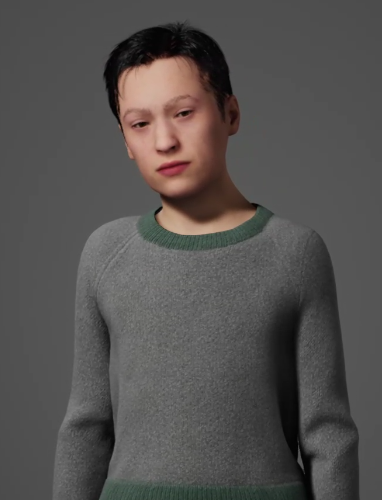
\includegraphics[width=0.6\textwidth]{chapters/conclusion/images/metahuman_bazeel.png}
    \caption{MetaHuman BAZeel}
    \label{fig:conclusion:metahuman_bazeel}
\end{figure}

\subsection{AZVD}
\label{ch:conclusion:future:realistic_avatars}

The blender synthesizer was also integrated with the \gls{azvd}~\cite{filhol2024software} editor to generate \gls{sl} animations directly on a web interface (see Figure~\ref{fig:conclusion:azee_web_interface}).

\begin{figure}[ht]
    \centering
    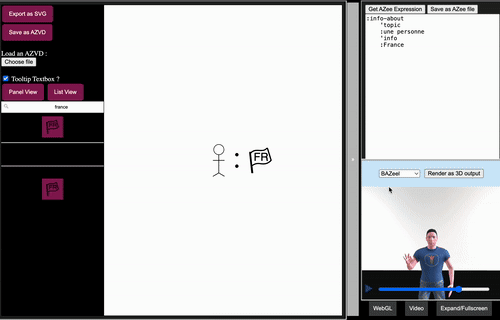
\includegraphics[width=0.9\textwidth]{chapters/conclusion/images/azee_web_interface.png}
    \caption{AZee web renderer interface}
    \label{fig:conclusion:azee_web_interface}
\end{figure}

The web interface allows users to draw \gls{azvd} which resolved to AZee Scores and then to animations. For this, the AZee code generated from \gls{azvd} in the front-end is sent to the server where an instance of the blender is running headlessly. The synthesizer evaluates the AZee code and returns the animation in video or GLB format to the front-end where it is displayed to the user. However, the system only supports a few AZee rules for now. A complete system, when integrated with more AZee rules could allow us to draw \gls{sl} discourses and will serve as a strong tool in empowering the language.

\end{document}